\documentclass[9pt, aspectratio=43, english]{beamer}

\graphicspath{{./graphics/}}

\usetheme[style=fwn]{leidenuniv}

\usepackage{dsfont}
\usepackage{amsmath}
\newcommand{\N}{\mathds{N}}

% uncomment next line to let framesubtitle have palette primary color
%\setbeamercolor{framesubtitle}{use={palette primary},fg=palette primary.bg}

% uncomment next line to remove navigation symbols from the pdf
%\setbeamertemplate{navigation symbols}{}

\title{Accessing Leiden via bus}
\subtitle{}
\author{Jeroen Ockers}
\institute{Universiteit Leiden}
\date{May 28th, 2025}
\titlegraphic{
	
\includegraphics[height=0.3\paperheight]{logo-universiteitleiden-english.pdf}
}


\begin{document}
% ====================================================================

% --------------------------------------------------------------------

\setbeamertemplate{navigation symbols}{}
\begin{frame}[plain]
  \maketitle
\end{frame}
\addtocounter{framenumber}{-1}% don't count the title slide.


% --------------------------------------------------------------------
\begin{frame}{Table of Contents}
  \tableofcontents[sectionstyle=show/show, hideallsubsections]
\end{frame}


% ====================================================================
\section{Introduction}
\begin{frame}{Make Leiden more accesible}
  \begin{itemize}
    \item Less mobile people
    \item Encourage bus use
  \end{itemize}
\end{frame}

\begin{frame}{Rumpf and Kaul}
  \begin{columns}
    \begin{column}{0.48\textwidth}
      \begin{itemize}
        \item Origin - Destination points
        \item Small increase in cost
      \end{itemize}
    \end{column}

    \begin{column}{0.48\textwidth}
    \begin{figure}
      \centering
      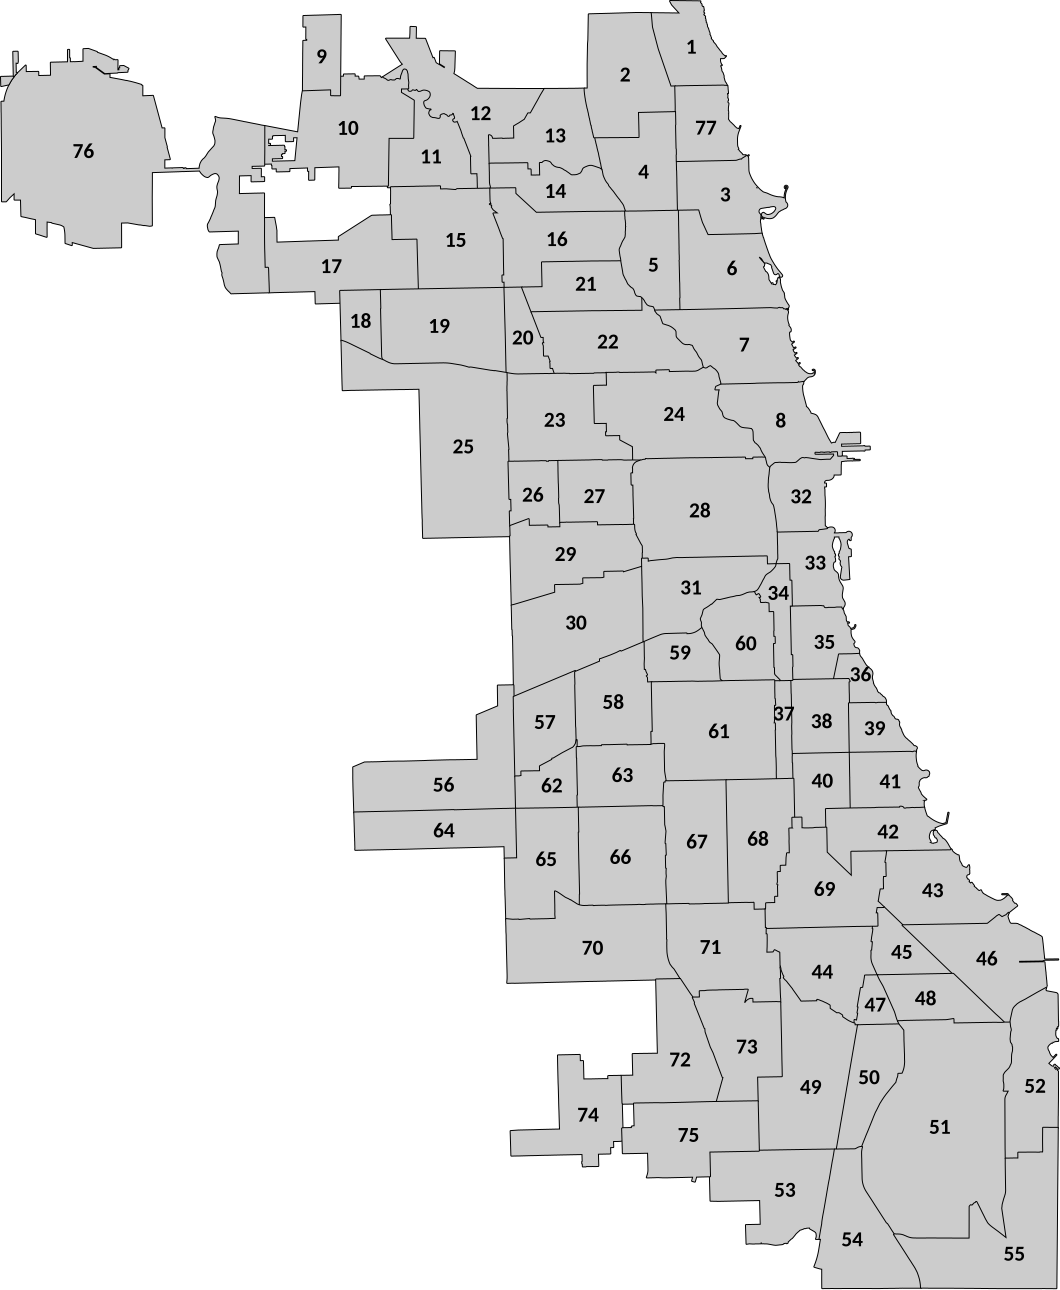
\includegraphics[width=\textwidth]{Chicago_Community_Areas.png}
    \end{figure}
    \end{column}
  \end{columns}
\end{frame}
% ====================================================================
\section{Applying the algorithm}
% ====================================================================
\begin{frame}
  \frametitle{Applying the algorithm}

  Data required:
  \begin{itemize}
    \item <1->Destinations
    \item <2->Origins
    \item <3->Busstop locations
    \item <4->Current bus schedule
    \item <5->Current travel data
  \end{itemize}

\end{frame}


\begin{frame}
  \frametitle{Destinations}
  \begin{itemize}
    \item GP locations
    \item Quality 
    \item No hospitals
  \end{itemize}

\end{frame}
\subsection{PC4}


\subsection{Voronoi}


% ====================================================================
\section{Next steps}
\begin{frame}{Next steps}
    \begin{itemize}
        \item asdf
    \end{itemize}
\end{frame}

\end{document}





